
\chapter{Configure Horizon}
In this section, we will Configure OpenStack Dashboard Service, wihch is the service for monitoring and managing other services using a UI (Horizon).
%Intro\footnotemark\\
\begin{spacing}{1.2}
%note en bas de page

\section{Installing Horizon}
\par Installing Horizon service using the dnf package manager.
\\
\begin{figure}[!htb] 
\begin{center} 
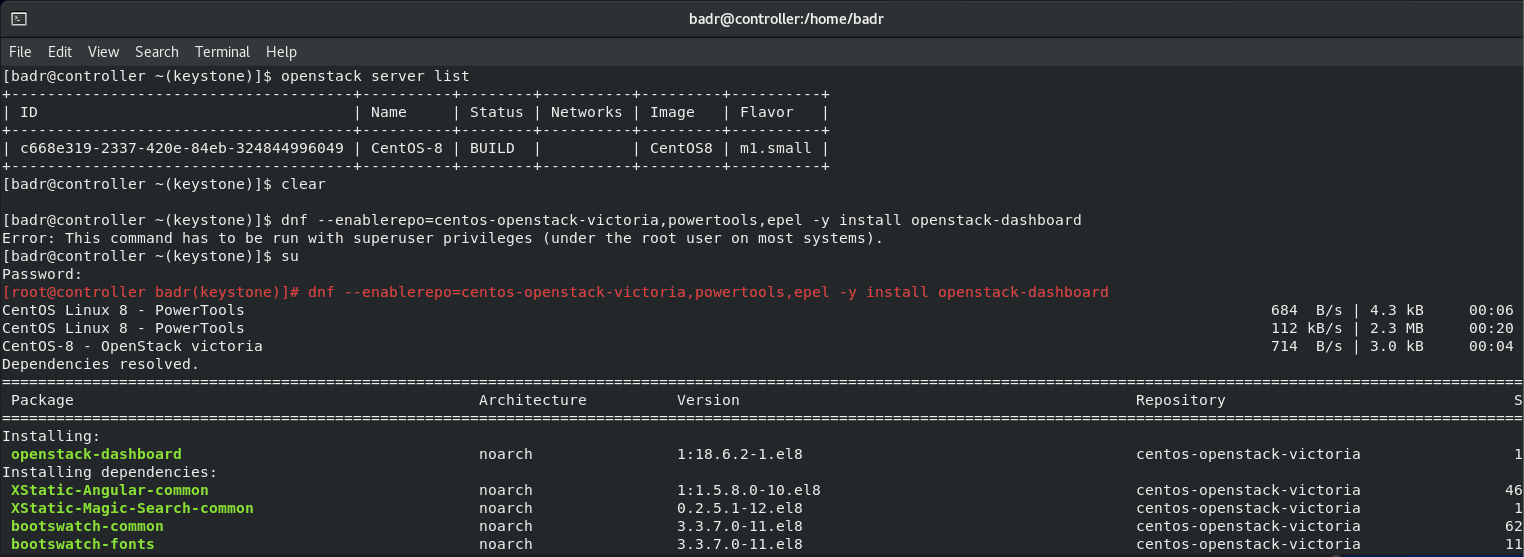
\includegraphics[width=1\linewidth]{Cloud/Configure Horizon/C_1.png} 
\end{center} 
\caption{ Horizon installation} 
\end{figure} 
\FloatBarrier
\\
\section{Horizon Configuration}
\par Setting the hosts that can use Horizon dashboard, here we set * which is everyone and we remove the other line.
\\
\begin{figure}[!htb] 
\begin{center} 
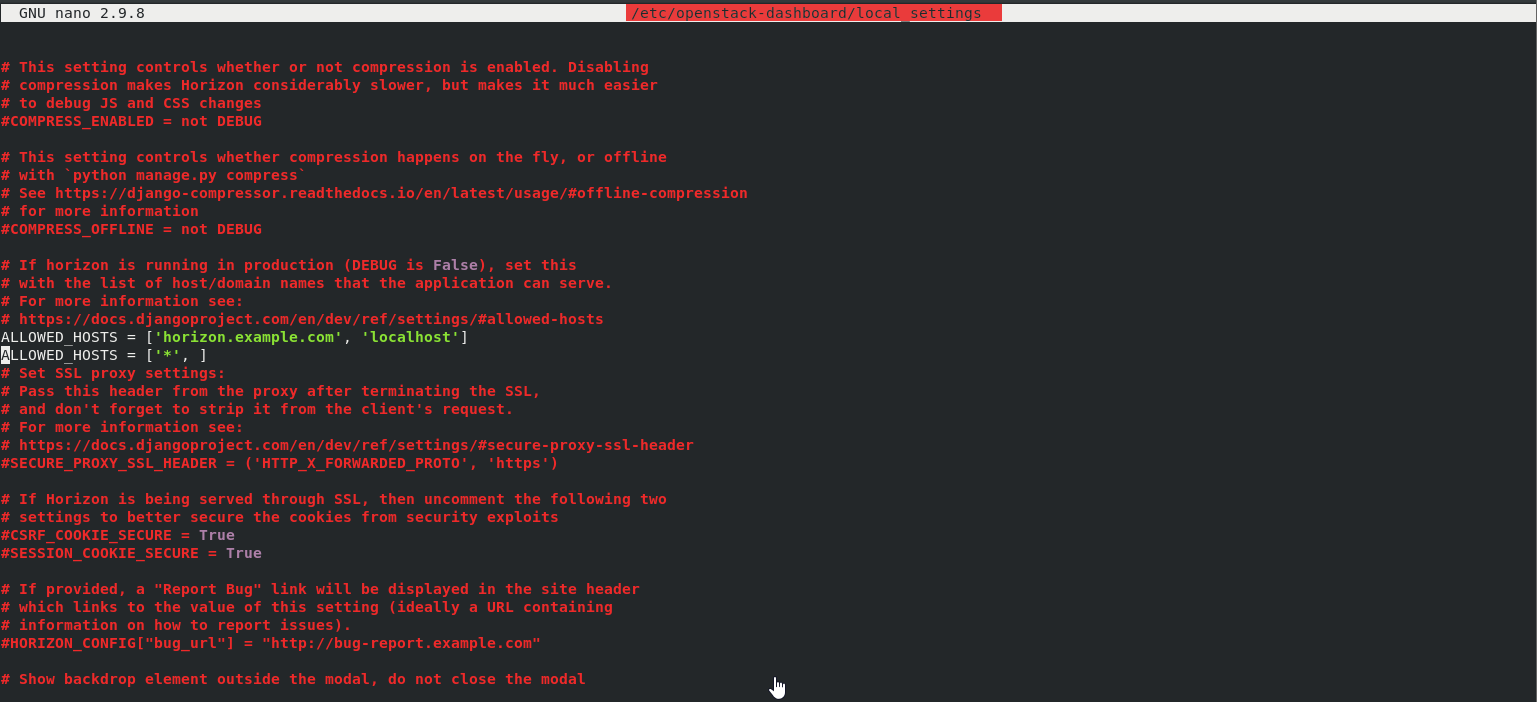
\includegraphics[width=1\linewidth]{Cloud/Configure Horizon/C_2_conf_1.png} 
\end{center} 
\caption{ Horizon Configuation: } 
\end{figure} 
\FloatBarrier
\\

\par In the Green Selection: we are setting the cache location and which implementation to use for caching, here we use Memecached library in Django since our dashboard use Django as the back-end. 
\\
\par in the Yellow Selection: we are setting a secret key for the Dashboard API.
\\
\begin{figure}[!htb] 
\begin{center} 
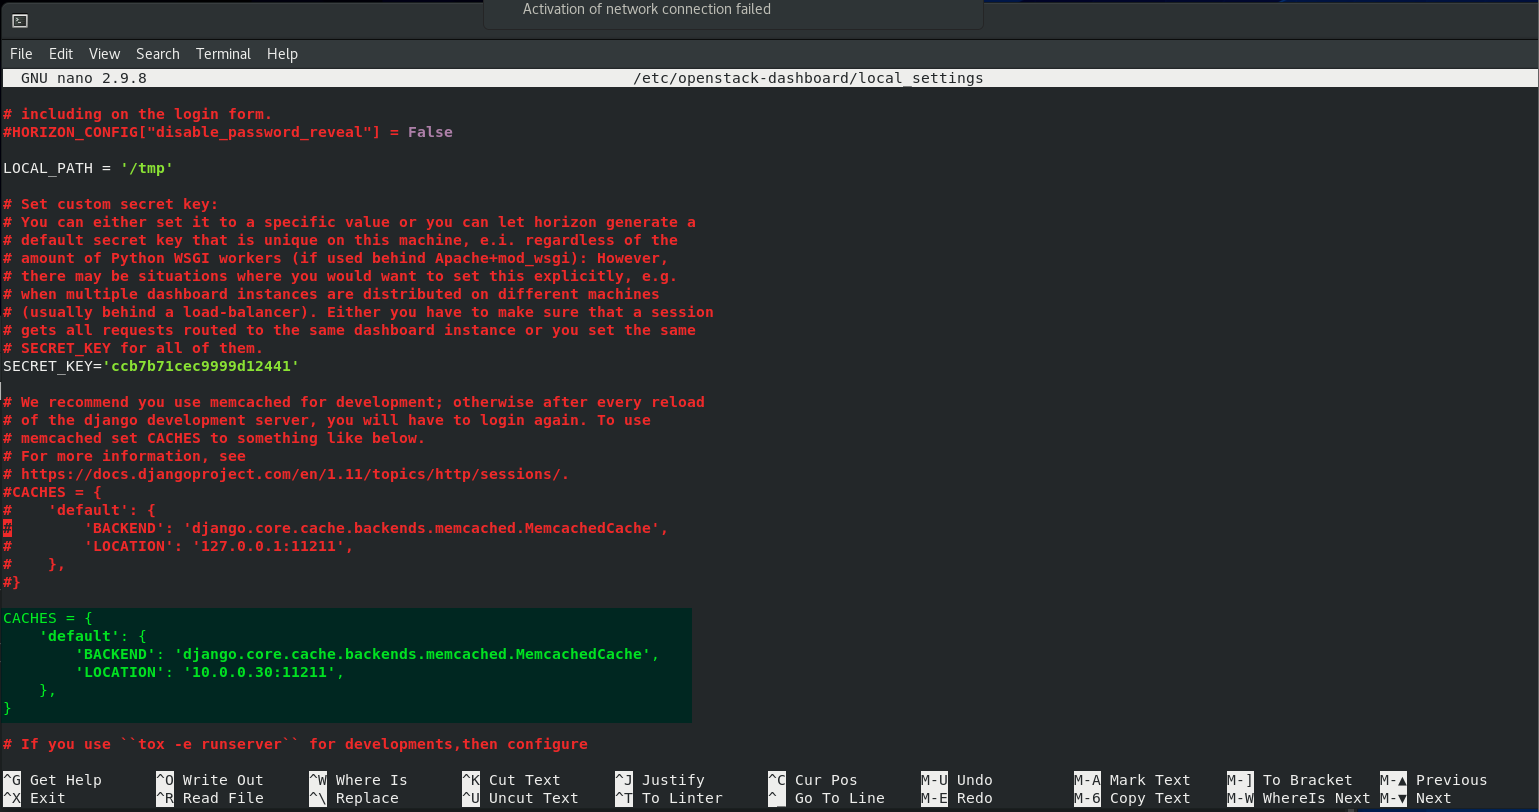
\includegraphics[width=1\linewidth]{Cloud/Configure Horizon/C_2_conf_2.png} 
\end{center} 
\caption{ Horizon configuration:Cache configuration} 
\end{figure} 
\FloatBarrier
\\
\par In the Yellow Selection: some additional caching configuration.
\par In the Green Selection: we define the the timezone and Openstack host that the dashboard will connect to and use.
\\

\\
\begin{figure}[!htb] 
\begin{center} 
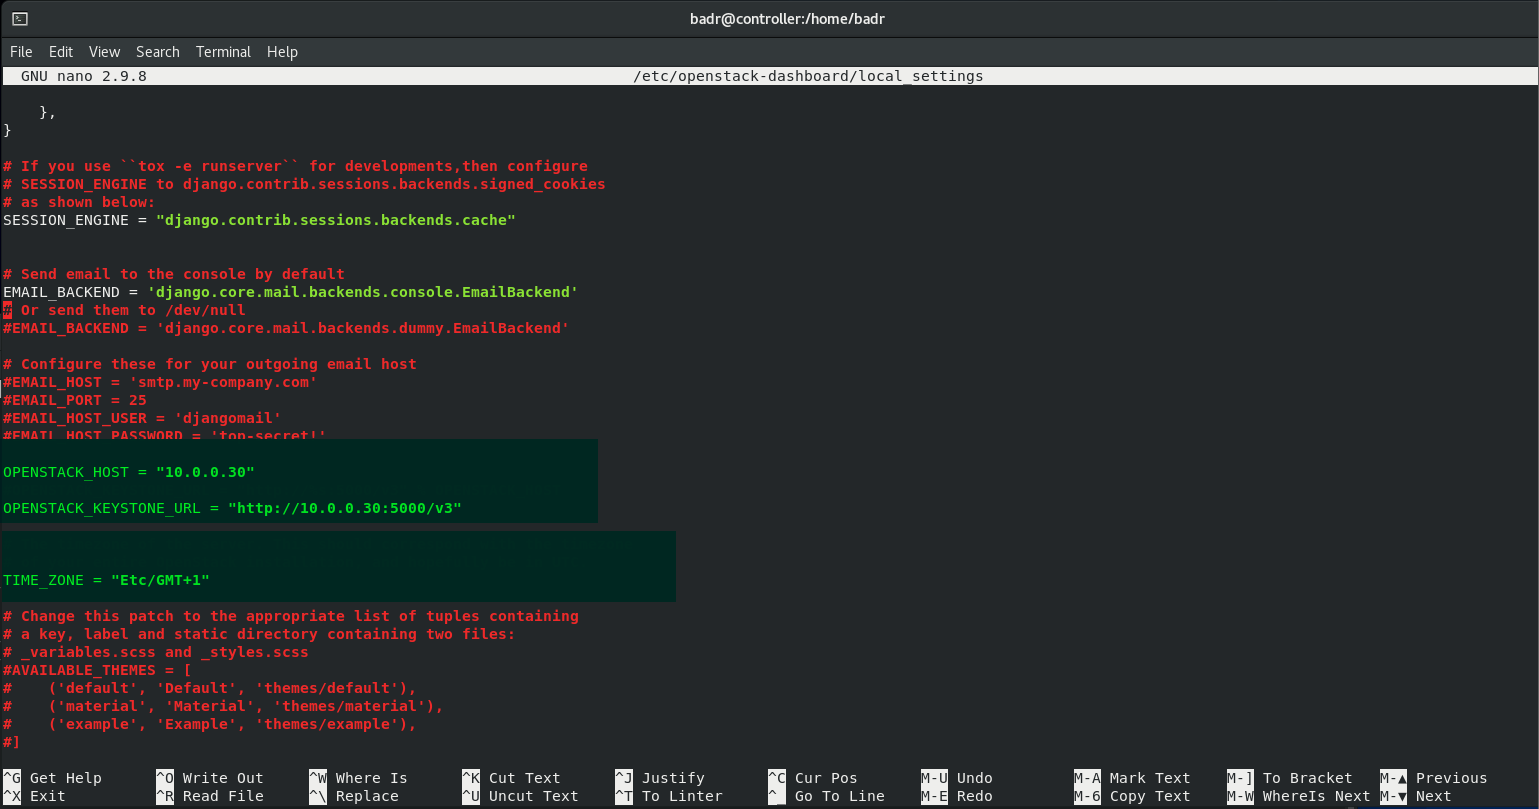
\includegraphics[width=1\linewidth]{Cloud/Configure Horizon/C_2_conf_3.png} 
\end{center} 
\caption{ Horizon configuration: Openstack caching, host and timezone} 
\end{figure} 
\FloatBarrier
\\
\par In the Yellow Selection: We define the connection protocols and the ports to use for some connection, for example MY SQL will use a tcp on port 3306 so Horizon will try to establish a connection on this port using tcp in order to make use of Mysql.

\par In the Green Selection: we define the URI'S for our dashboard, so we can give the used simple endpoint and then redirecting him to one that the dashboard use.
\\
\begin{figure}[!htb] 
\begin{center} 
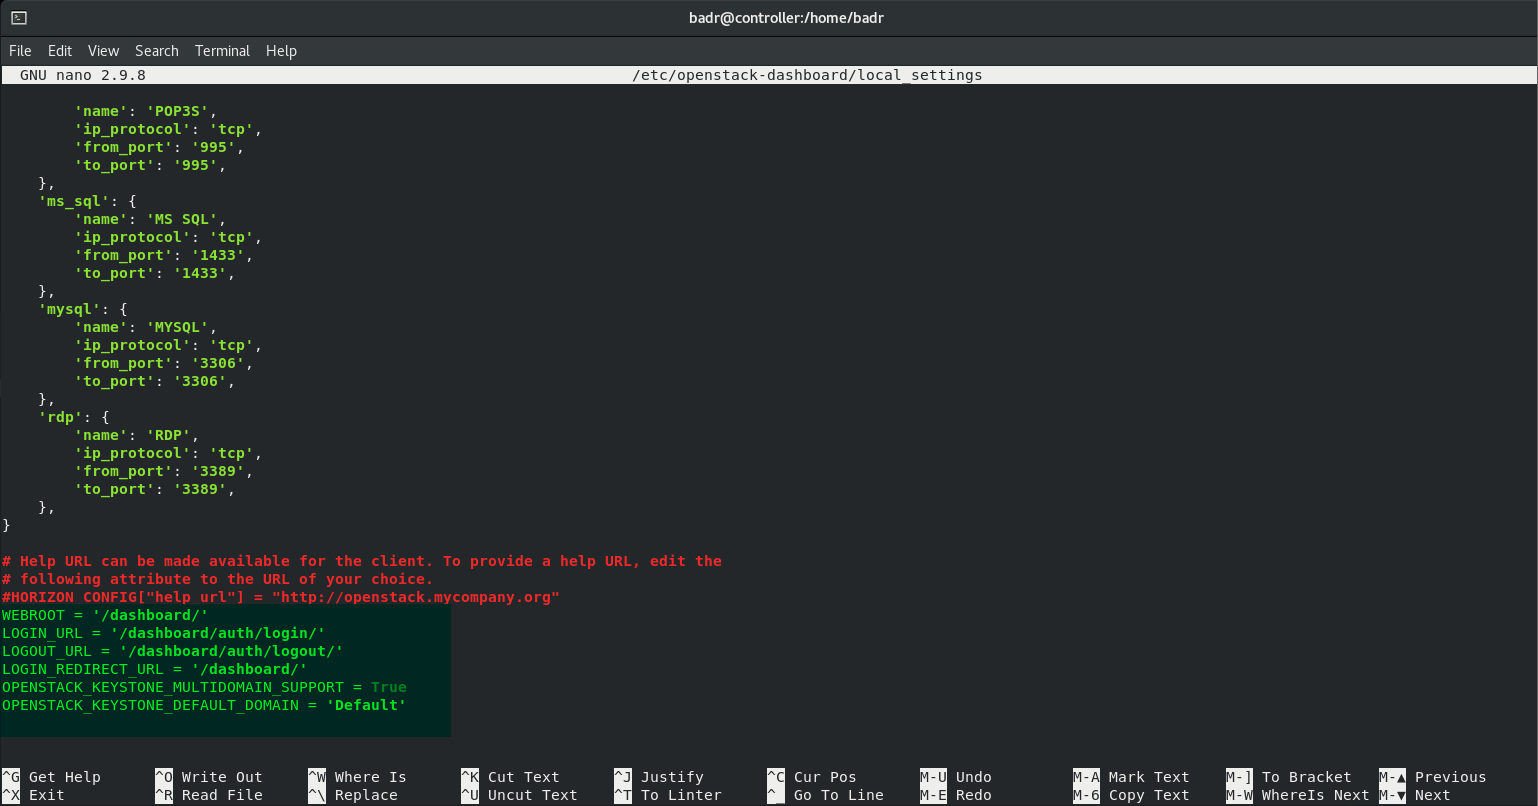
\includegraphics[width=1\linewidth]{Cloud/Configure Horizon/C_2_conf_4.png} 
\end{center} 
\caption{ Horizon configuration} 
\end{figure} 
\FloatBarrier
\\

\par Defining the SQL application group parameter to use a global variable.
\\
\begin{figure}[!htb] 
\begin{center} 
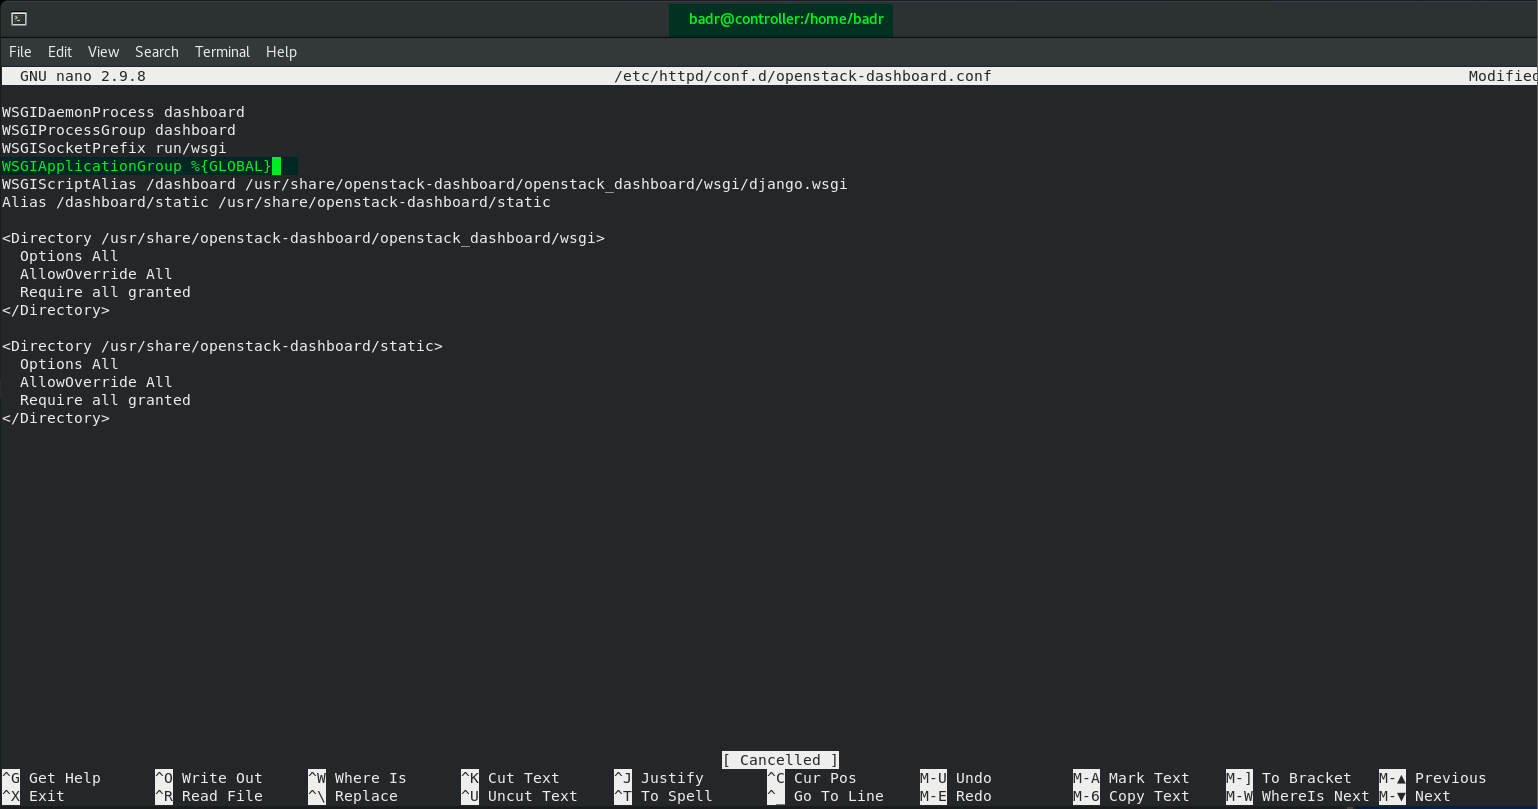
\includegraphics[width=1\linewidth]{Cloud/Configure Horizon/C_3_conf_5.png} 
\end{center} 
\caption{ Horizon configuration} 
\end{figure} 
\FloatBarrier
\\

\par Restarting the http in order to apply changes.
\\
\begin{figure}[!htb] 
\begin{center} 
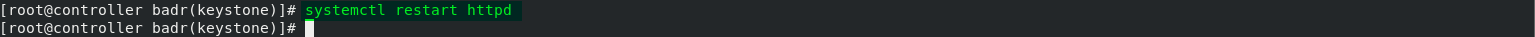
\includegraphics[width=1\linewidth]{Cloud/Configure Horizon/C_4.png} 
\end{center} 
\caption{ restart httpd service} 
\end{figure} 
\FloatBarrier
\\

\par Adding new roles to nova, that horizon dashboard will be using.
\\
\begin{figure}[!htb] 
\begin{center} 
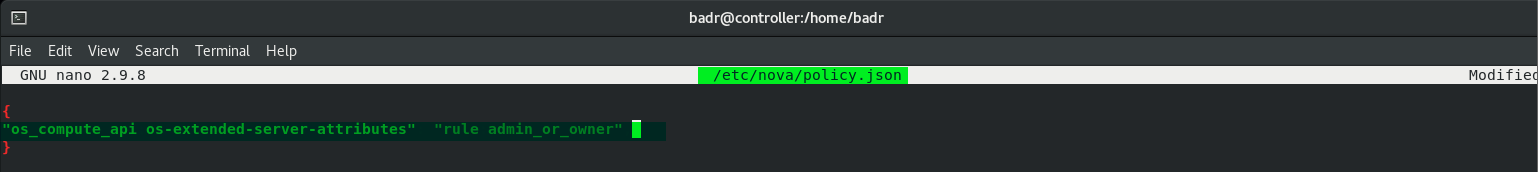
\includegraphics[width=1\linewidth]{Cloud/Configure Horizon/C_5.png} 
\end{center} 
\caption{ Adding new roles to nova policy} 
\end{figure} 
\FloatBarrier
\\

\par restarting opan-stack-nova-api in order to apply changes made to policy
\\
\begin{figure}[!htb] 
\begin{center} 
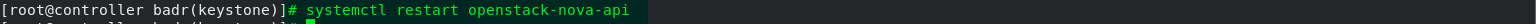
\includegraphics[width=1\linewidth]{Cloud/Configure Horizon/C_6.png} 
\end{center} 
\caption{ Restarting pan-stack-nova-api service} 
\end{figure} 
\FloatBarrier
\\
\newpage
\section{Accessing the dashboard}
\par Now we will access our horizon dashboard, for the credentials we use the same ones as we did in the configuration, for the domain we use default and for the User name and password we use the ones in the keystone; since keystone is the service that provide service discovery and authentication.
\\
\begin{figure}[!htb] 
\begin{center} 
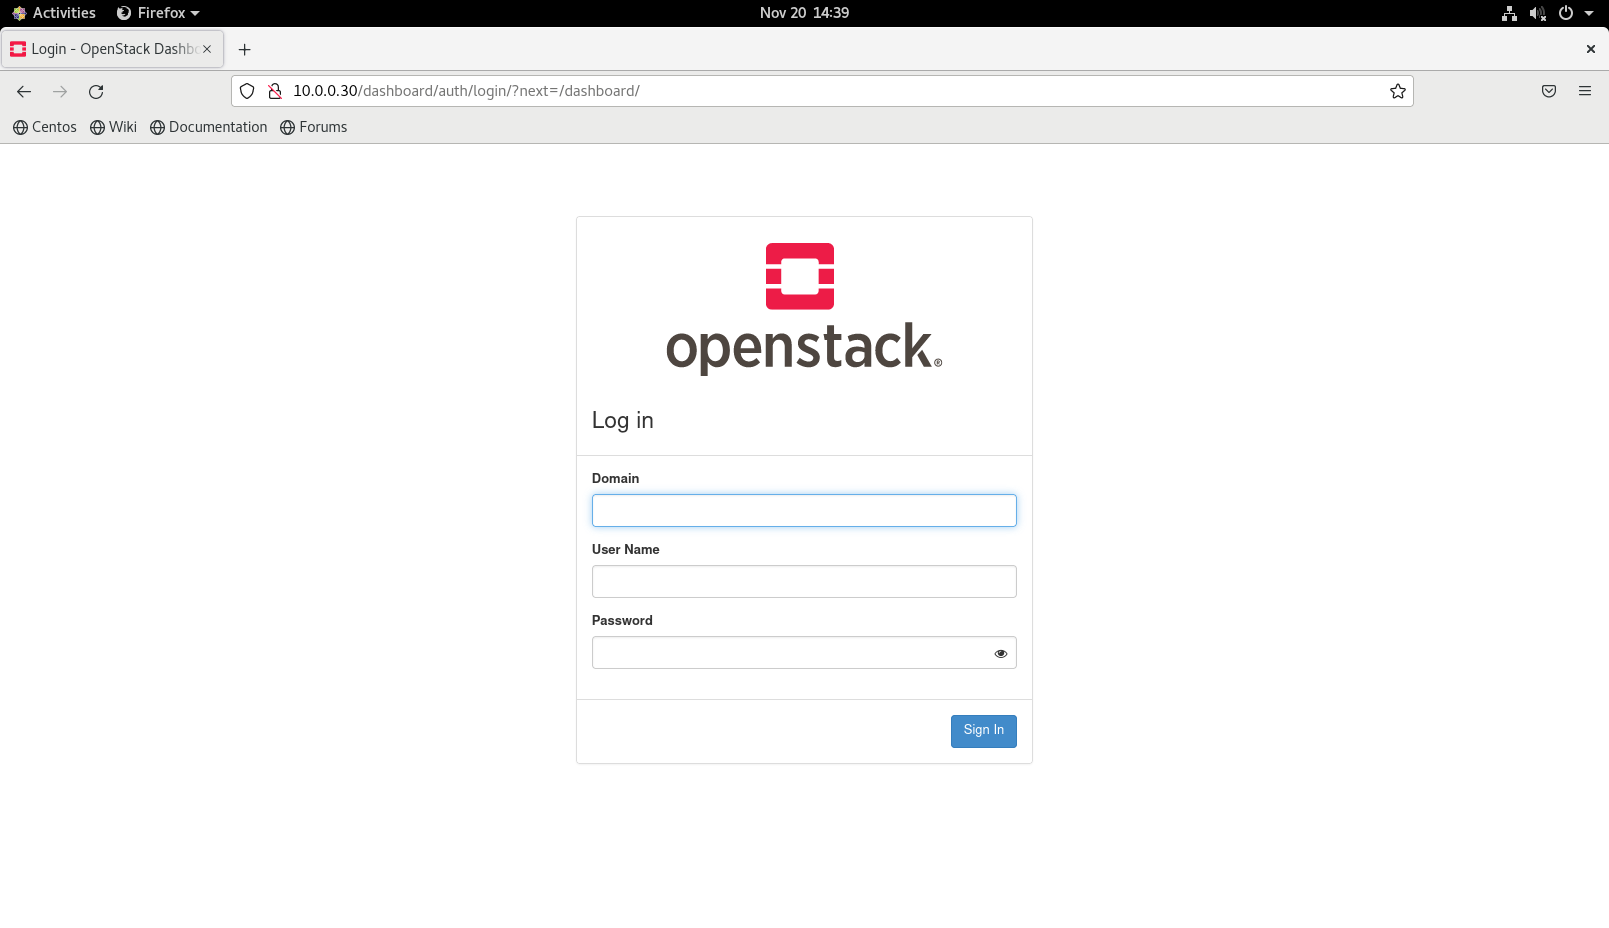
\includegraphics[width=1\linewidth]{Cloud/Configure Horizon/C_7.png} 
\end{center} 
\caption{  Login to the dashboard} 
\end{figure} 
\FloatBarrier
\\

\par Our dashboard shows 0 instance, since our instance is always \textbf{stuck at the build state} and keep building rather to pass to the Active status.
\\
\begin{figure}[!htb] 
\begin{center} 
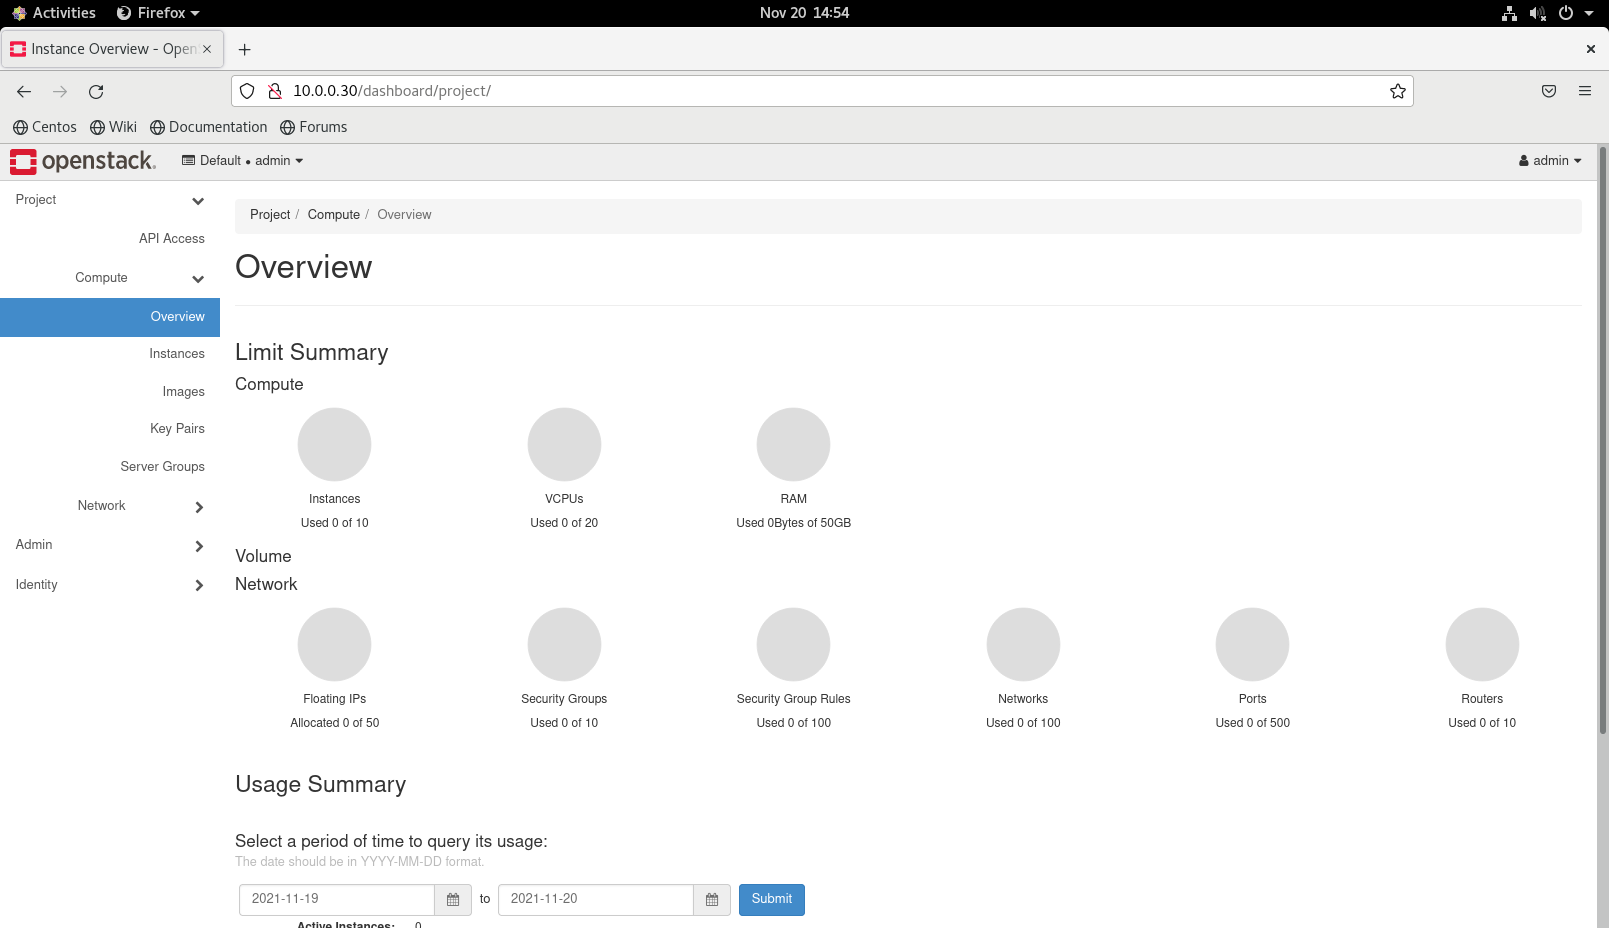
\includegraphics[width=1\linewidth]{Cloud/Configure Horizon/C_8.png} 
\end{center} 
\caption{  Horizon dashboard} 
\end{figure} 
\FloatBarrier
\\

\par Since our instance is always stuck at the BUILD status we couldn't visualise any instance, so we will discuss only the \textbf{expected result}. As shown in the figure 10.12 we can see all active instances and interact whit them; deleting them stopping them etc etc...
\\
\begin{figure}[!htb] 
\begin{center} 
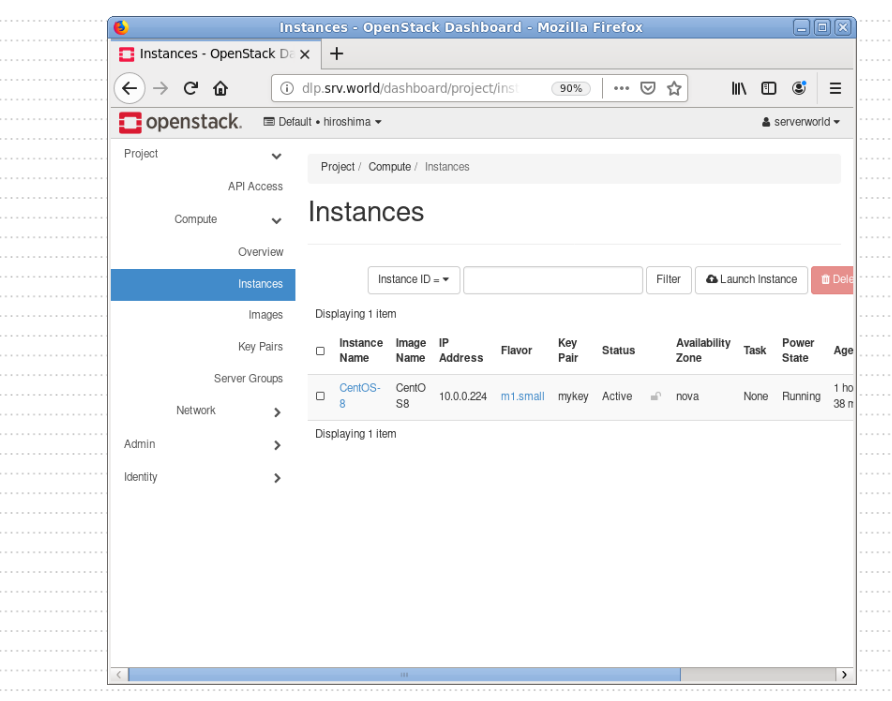
\includegraphics[width=1\linewidth]{Cloud/Configure Horizon/C_9_expected_results.png} 
\end{center} 
\caption{  Expected result} 
\end{figure} 
\FloatBarrier

\begin{figure}[!htb] 
\begin{center} 
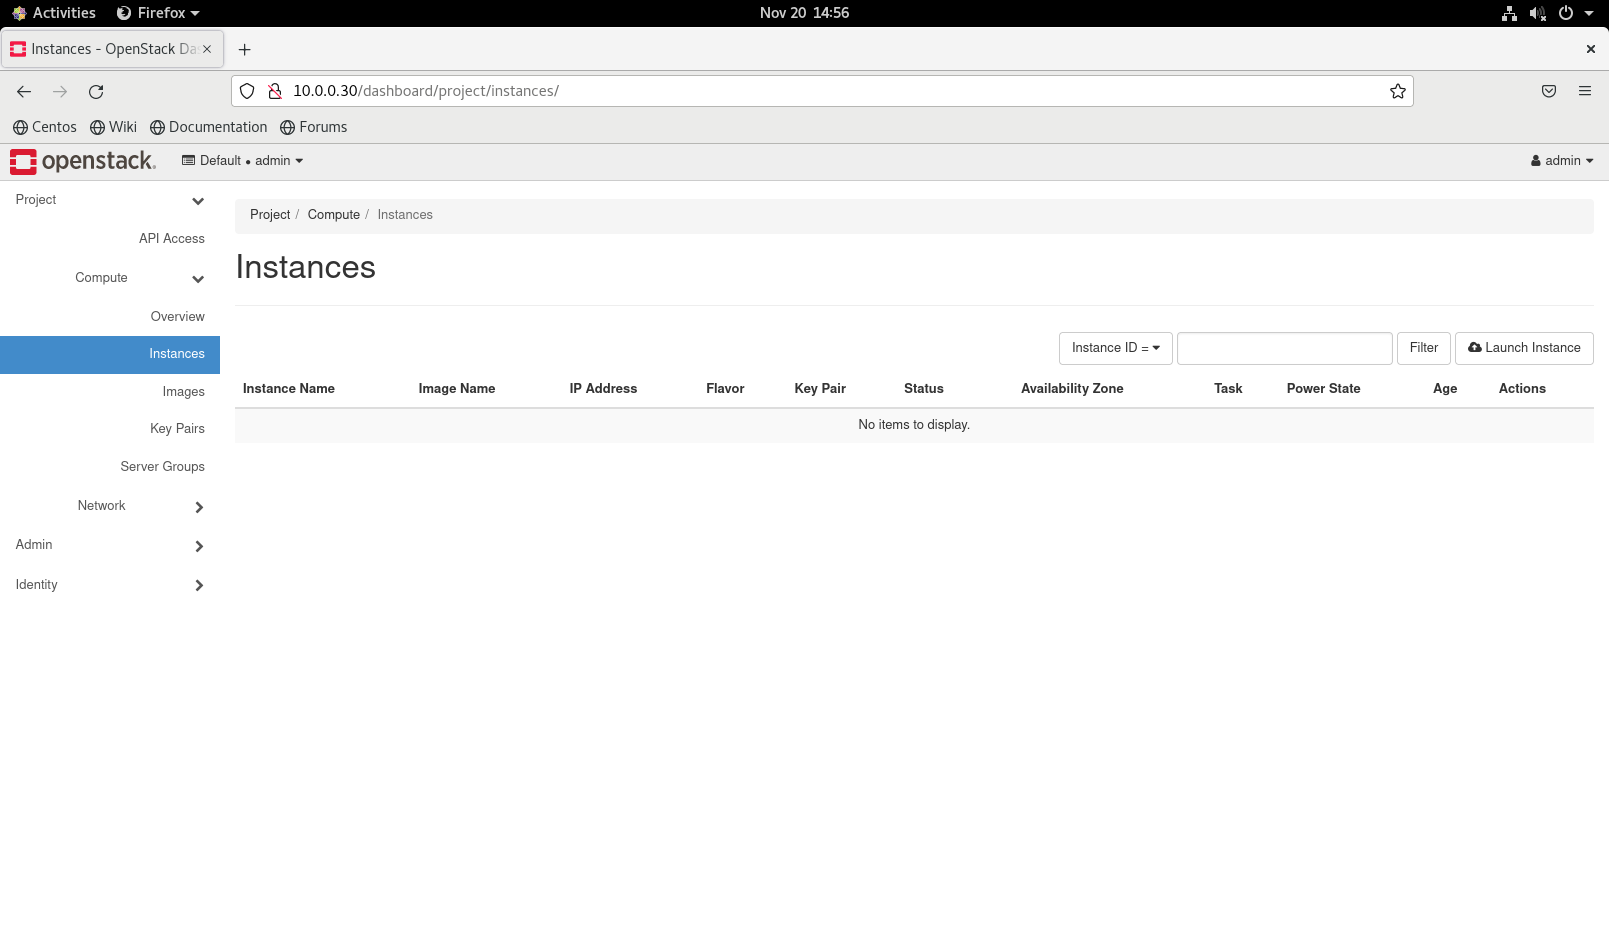
\includegraphics[width=1\linewidth]{Cloud/Configure Horizon/C_9_our result because our instance is always stuck at building state.png} 
\end{center} 
\caption{  Our result} 
\end{figure} 
\FloatBarrier
\\

\par Just to ensure that \textbf{our horizon service is working}, and our problem is only about the server instance stuck at build status, we can see other services like the images service(glance), here we can see our Cent-OS08 image that we created at step-6, thus our horizon service is working.
\\
\begin{figure}[!htb] 
\begin{center} 
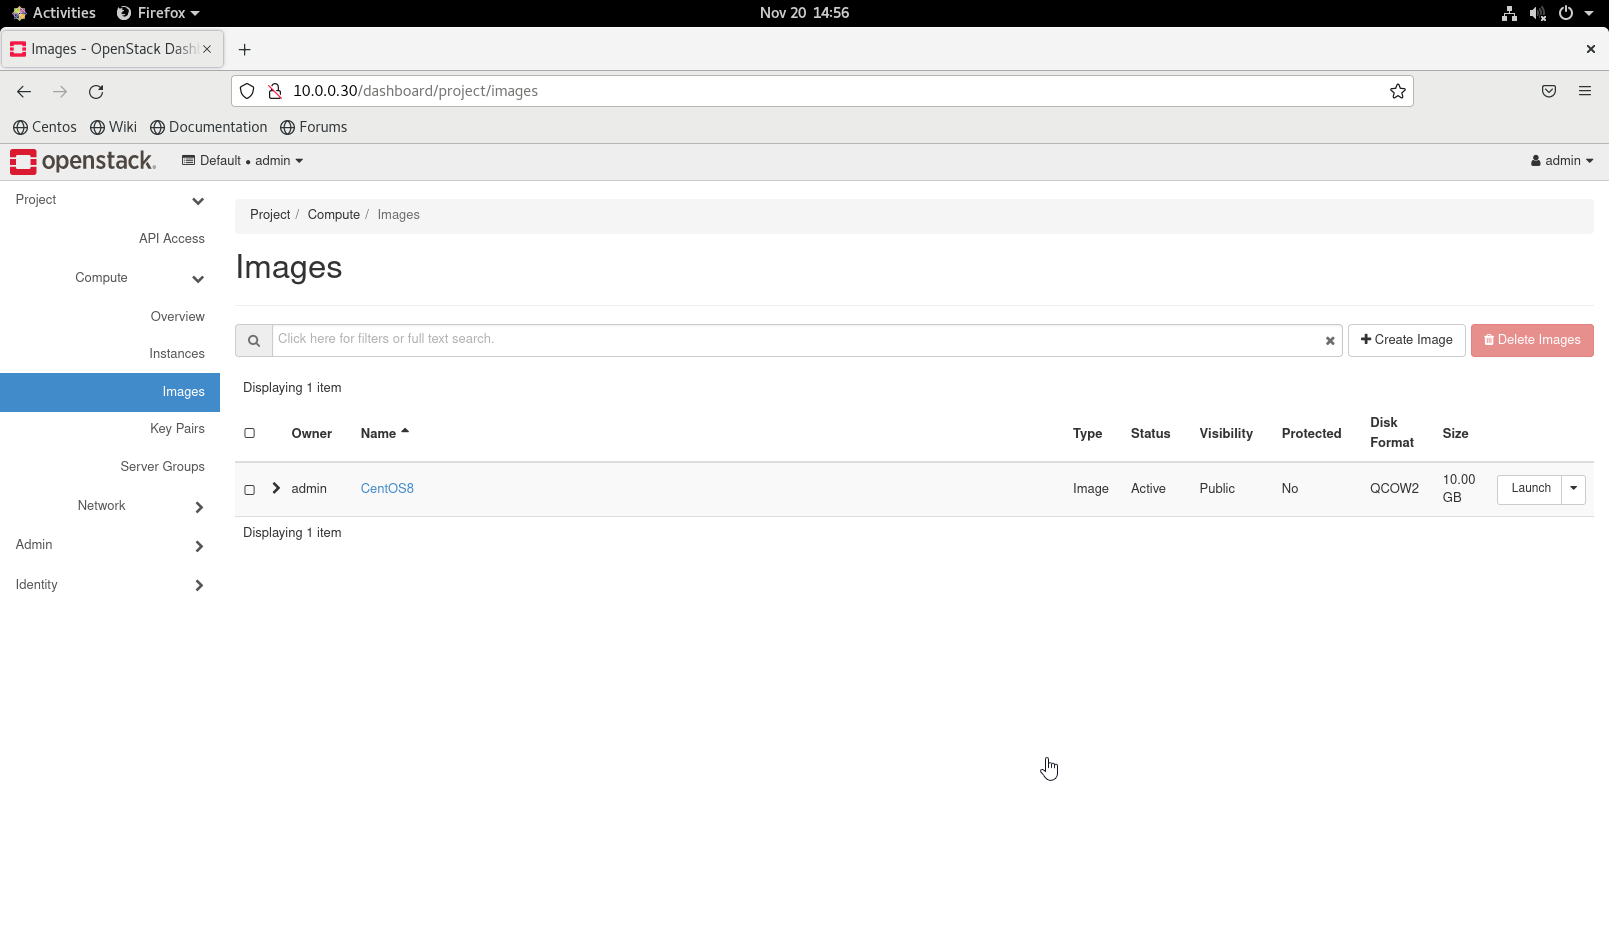
\includegraphics[width=1\linewidth]{Cloud/Configure Horizon/C_9_proof of correctness since we can see the images we created we can say that horizon service is working.png} 
\end{center} 
\caption{  Proof that Horizon is working.} 
\end{figure} 
\FloatBarrier
\\

\par Using horizon dashboard we can see more detailed information about our instance and also connect using the VNC whit only a one click, keep in mind that theses result are not ours it's only the expected result since our server instance is always stuck at building status.
\\
\begin{figure}[!htb] 
\begin{center} 
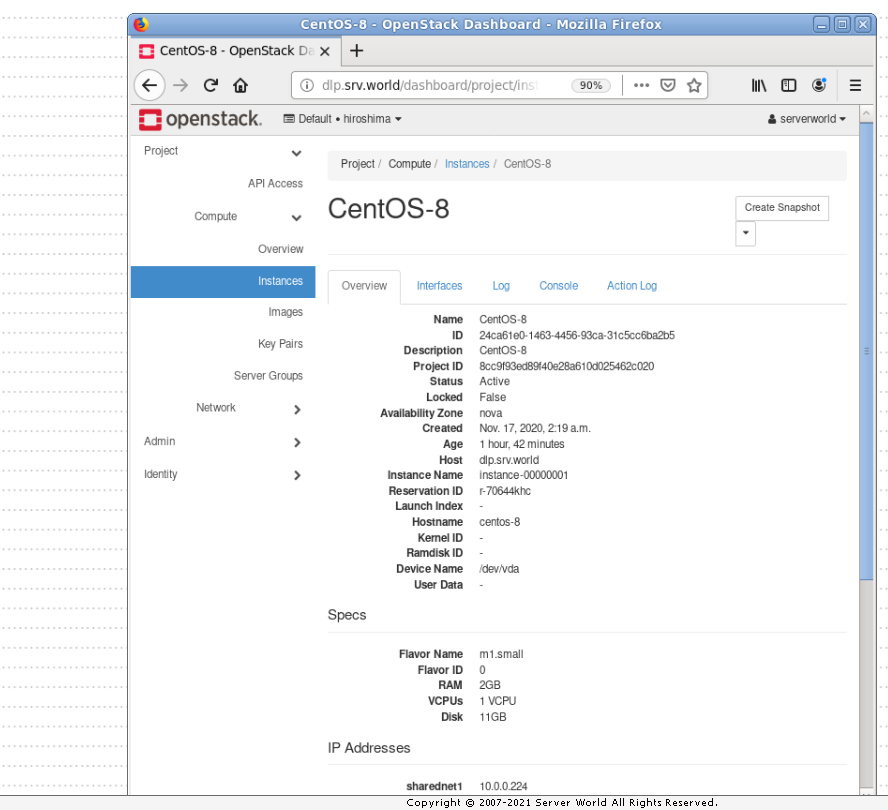
\includegraphics[width=1\linewidth]{Cloud/Configure Horizon/C_10_expected result, since our instance is always at the building state we can't see this page.png} 
\end{center} 
\caption{  Horizon dashboard: information about instances (Expected result)} 
\end{figure} 
\FloatBarrier
\\


\begin{figure}[!htb] 
\begin{center} 
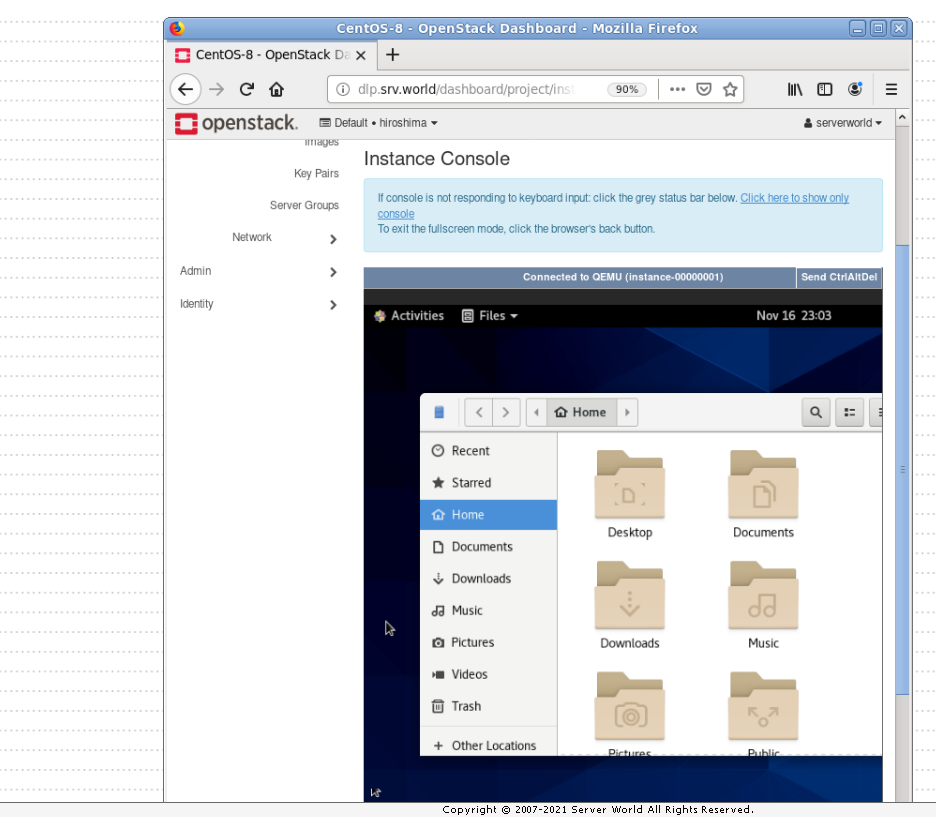
\includegraphics[width=1\linewidth]{Cloud/Configure Horizon/C_11_expected result, since our instance is always at the building state we can't establish the ssh connection.png} 
\end{center} 
\caption{  VNC using browser (Expected result)} 
\end{figure} 
\FloatBarrier
\\
\end{spacing}